  % hahaha
  %% diplomarbeit.tex
  %% Copyright 2015 Simon M. Laube
  %
  % This work may be distributed and/or modified under the
  % conditions of the LaTeX Project Public License, either version 1.3
  % of this license or (at your option) any later version.
  % The latest version of this license is in
  %   http://www.latex-project.org/lppl.txt
  % and version 1.3 or later is part of all distributions of LaTeX
  % version 2005/12/01 or later.
  %
  % This work has the LPPL maintenance status `author maintained'.
  % 
  % The Current Maintainer of this work is S. M. Laube
  %
  % This work consists of the files listed in ./Help/files.txt

%%=====================================================%%
%% Neues Diplomarbeitstemplate der ET	   			   %%
%% Abteilung ab 2013/2014				   			   %%
%% Erstellt von Simon Michael Laube		   			   %%
%% Betreut von  Prof. Mag. Dipl.-Ing. Dr. Daniel Asch  %%
%%			    Prof. Dipl.-Ing. Dr. Wilhelm Haager	   %%
%%=====================================================%%
%% Dokumentklasse KOMA-Script Report
\documentclass[paper=a4,12pt]{scrreprt}
% Encoding UTF8
\usepackage[utf8]{inputenc}
% 8 Bit Aufloesung der Buchstaben
\usepackage[T1]{fontenc}
% Seitenraender
\usepackage[scale=0.72]{geometry}
% Spracheinstellungen
\usepackage[english, naustrian]{babel} % your native language must be the last one!!
% erweiterte Farbenpalette
\usepackage[dvipsnames]{xcolor}
% Abbildungen
\usepackage{graphicx}
% Tabellen (erweitert)
\usepackage{tabularx}
% TikZ + Circuit-TikZ (fuer Schaltungen)									
\usepackage[europeanresistors,							
			europeaninductors]{circuitikz}
% Nuetzliche TikZ Libraries
\usetikzlibrary{arrows,automata,positioning}
% Mathematikpakete!
\usepackage{amsmath,amssymb}							
%\usepackage{mathtools}	
% PDF Einbindung (zB Datenblaetter)
\usepackage{pdfpages}
% Source Code Einbindung, Setup siehe:
% http://en.wikibooks.org/wiki/LaTeX/Source_Code_Listings									
\usepackage{listings,scrhack} %scrhack vermeidet Umschaltung auf KOMA Floats..			
% Ausrichtung der Bilder
\usepackage[export]{adjustbox}

% The Euro­pean cur­rency sym­bol for the Euro			
\usepackage{eurosym}

% Landscape
\usepackage{lscape}
\usepackage{tabularx}
% Diplomarbeitsspezifisches Package etdipa
\usepackage{etdipa}

%% Abkuerzungsverzeichnis
\usepackage[]{acronym}
\usepackage{xcolor}
%% Todos
\usepackage[]{todonotes}

%% Ganttdiagramme
\usepackage{pgfgantt}
\usepackage{xcolor}
\usepackage{graphics}
\usepackage{graphicx}
\usepackage{capt-of}
%% Subfigures
\usepackage[lofdepth]{subfig}


%%==== Definitionen fuer die Diplomarbeit ============%%
\dokumenttyp{DIPLOMARBEIT}
\title{Musterdokument}
\author{Hans Huber \and Birgit Bauer}
\date{\today}
\place{Mödling}
\schuljahr{2018/19}
\professor{Prof. Rick}
\dipacolor{ETred}
%%====================================================%%


% Hyperlinks im Dokument
\usepackage[colorlinks=true,
			linkcolor=black,
			citecolor=black,
			bookmarks=true,
			urlcolor=black,
			bookmarksopen=true]{hyperref}
\begin{document}

\frontmatter

%%================ Titelseite ==========================%%
\maketitle
% Verantwortliche/Verfasser
%%======================================================%%

%%================ Eidesstattliche Erklaerung ==========%%

\begin{Eid}%Unterschrift der Diplomanden hinzufuegen!
\unterschrift{Hans Huber}
\unterschrift{Birgit Bauer}

\end{Eid}\newpage
%%======================================================%%

%%================ Diplomandenvorstellung ==============%%
%% start of file diplomanden.tex

%% Diplomandenvorstellung:
\begin{Diplomandenvorstellung}
%% Schueler1 
\diplomand{Hans Huber}
		  {12.12.2012 in Mödling}
		  {Hauptstra\ss e 13}
		  {2340 Mödling}
		  {\schule{2010--2015}{HTBLuVA Mödling, Abteilung für Elektrotechnik und Technische Informatik}
		  \schule{2006--2010}{Gymnasium XY}}
		  {hans.huber@xy.at}
		  {Images/latex3}
\newpage	  
%% Schueler2
\diplomand{ Birgit Bauer}
		  {12.12.2012 in Wien}
		  {Langestra\ss e 14}
		  {1230 Wien}
		  {\schule{2010--2015}{HTBLuVA Mödling, Abteilung für Elektrotechnik und Technische Informatik}
		   \firma{2006--2010}{Elektrofirma XY}
		   \schule{2002--2006}{Gymnasium XY}}
		  {birgit.bauer@xy.at}
		  {Images/latex}

\newpage	  
\end{Diplomandenvorstellung}

%% end of file diplomanden.tex

%%======================================================%%

%%================ Tabelle ==============%%
\begin{center}
	\large \textbf {Diplomarbeit \\ Dokumentation} \normalsize
\end{center}

\noindent
\begin{tabularx}{\textwidth}{|m{0.35\textwidth}|X|}
	\hline
	Namen der Verfasser/innen & Namen \\
	\hline
	Jahrgang &  5BHEL\\
	Schuljahr & 2019/2020\\
	\hline
	Thema der Diplomarbeit& Thema\\
	\hline
	Kooperationspartner & Sponsoren\\
	\hline

\end{tabularx}
\\
\\
\\
\noindent
\begin{tabularx}{\textwidth}{|m{0.35\textwidth}|X|}
	\hline
 	Aufgabenstellung & //Text \\
 	&\\
 	&\\
 	&\\
 	&\\
 	&\\
 	&\\
 	&\\
 	
	\hline
	
\end{tabularx}
\\
\\
\\
\noindent
\begin{tabularx}{\textwidth}{|m{0.35\textwidth}|X|}
	\hline
	Realisierung & //Text \\
	&\\
	&\\
	&\\
	&\\
	&\\
	&\\
	&\\
	
	\hline
	
\end{tabularx}
\\
\\
\\
\noindent
\begin{tabularx}{\textwidth}{|m{0.35\textwidth}|X|}
	\hline
	Ergebnisse & //Text \\
	&\\
	&\\
	&\\
	&\\
	&\\
	&\\
	
	\hline
	
\end{tabularx}
\\
\\
\\
\noindent
\begin{tabularx}{\textwidth}{|m{0.35\textwidth}|X|}
	\hline
	Typische Grafik, Foto, etc. & //Text \\
	(mit Erläuterung)&\\
	&\\
	&\\
	&\\
	&\\
	&\\
	
	\hline
	
\end{tabularx}
\\
\\
\\
\noindent
\begin{tabularx}{\textwidth}{|m{0.35\textwidth}|X|}
	\hline
	Teilnahme an Wettbewerben, Auszeichnungen & //Text \\
	&\\
	&\\
	&\\

	
	\hline
	
\end{tabularx}
\\
\\
\\
\noindent
\begin{tabularx}{\textwidth}{|m{0.35\textwidth}|X|}
	\hline
  	Möglichkeiten der Einsichtnahme in die Arbeit & Im Archiv der Abteilung Elektronik und Technische  Informatik der HTL Mödling \\
	&\\
	&\\
	&\\
	
	
	\hline
	
\end{tabularx}
\\
\\
\\
\noindent
\begin{tabularx}{\textwidth}{|c|r|Y|}
	\hline
	Approbation & \footnotesize{Prüfer/Prüferin} & Direktor/Direktorin \\
	\small{Date / Signature} \normalsize&  & \footnotesize{Abteilungsvorstand/Abteilungsvorständin} \\
	&&\\
	&&\\
	
	
	\hline
	
\end{tabularx}

\newpage

\begin{center}
	\large \textbf {Diploma Thesis \\ Docomentation} \normalsize
\end{center}

\noindent
\begin{tabularx}{\textwidth}{|m{0.35\textwidth}|X|}
	\hline
	Author(s) & Namen \\
	\hline
	Form &  5BHEL\\
	Academic year & 2019/2020\\
	\hline
	Topic& Thema\\
	\hline
	Co-operation partners & Sponsoren\\
	\hline
	
\end{tabularx}
\\
\\
\\
\noindent
\begin{tabularx}{\textwidth}{|m{0.35\textwidth}|X|}
	\hline
	Assignment of tasks & //Text \\
	&\\
	&\\
	&\\
	&\\
	&\\
	&\\
	&\\
	
	\hline
	
\end{tabularx}
\\
\\
\\
\noindent
\begin{tabularx}{\textwidth}{|m{0.35\textwidth}|X|}
	\hline
	Realisation & //Text \\
	&\\
	&\\
	&\\
	&\\
	&\\
	&\\
	&\\
	
	\hline
	
\end{tabularx}
\\
\\
\\
\noindent
\begin{tabularx}{\textwidth}{|m{0.35\textwidth}|X|}
	\hline
	Result & //Text \\
	&\\
	&\\
	&\\
	&\\
	&\\
	&\\
	
	\hline
	
\end{tabularx}
\\
\\
\\
\noindent
\begin{tabularx}{\textwidth}{|m{0.35\textwidth}|X|}
	\hline
	Illustrative graph, photo & //Text \\
	(incl. explanation)&\\
	&\\
	&\\
	&\\
	&\\
	&\\
	
	\hline
	
\end{tabularx}
\\
\\
\\
\noindent
\begin{tabularx}{\textwidth}{|m{0.35\textwidth}|X|}
	\hline
	Participation in competitions Awards & //Text \\
	&\\
	&\\
	&\\
	
	
	\hline
	
\end{tabularx}
\\
\\
\\
\noindent
\begin{tabularx}{\textwidth}{|m{0.35\textwidth}|X|}
	\hline
	Accessibility of Diploma Thesis & Stowed in the archive of the secondary technical college of Moedling, department of electronics and computer engineering \\
	&\\
	&\\
	&\\
	
	
	\hline
	
\end{tabularx}
\\
\\
\\
\noindent
\begin{tabularx}{\textwidth}{|c|r|Y|}
	\hline
	Approval & \footnotesize{ Examiner } & Head of College/Department \\
	\small{Date / Signature} &  & \\
	&&\\
	&&\\
	
	
	\hline
	
\end{tabularx}

%%======================================================%%

%%================ Danksagungen ========================%%
\newpage
%% start of file danksagungen.tex

%% Danksagungen:
\begin{Danksagung}
Wir bedanken uns bei \dots
\end{Danksagung}
\newpage

%% end of file danksagungen.tex
%%======================================================%%

%%================ Abstract /Zusammenfass. =============%%
%% start of file abstract.tex

\selectlanguage{english}
\begin{abstract}
Lorem ipsum dolor sit amet, consetetur sadipscing elitr, sed diam nonumy eirmod tempor invidunt ut labore et dolore magna aliquyam erat, sed diam voluptua. At vero eos et accusam et justo duo dolores et ea rebum. Stet clita kasd gubergren, no sea takimata sanctus est Lorem ipsum dolor sit amet. Lorem ipsum dolor sit amet, consetetur sadipscing elitr, sed diam nonumy eirmod tempor invidunt ut labore et dolore magna aliquyam erat, sed diam voluptua. At vero eos et accusam et justo duo dolores et ea rebum. Stet clita kasd gubergren, no sea takimata sanctus est Lorem ipsum dolor sit amet.
\end{abstract}
\selectlanguage{naustrian}

%% end of file abstract.tex
%% start of file zusammenfassung.tex

\selectlanguage{naustrian}
\begin{abstract}
Lorem ipsum dolor sit amet, consetetur sadipscing elitr, sed diam nonumy eirmod tempor invidunt ut labore et dolore magna aliquyam erat, sed diam voluptua. At vero eos et accusam et justo duo dolores et ea rebum. Stet clita kasd gubergren, no sea takimata sanctus est Lorem ipsum dolor sit amet. Lorem ipsum dolor sit amet, consetetur sadipscing elitr, sed diam nonumy eirmod tempor invidunt ut labore et dolore magna aliquyam erat, sed diam voluptua. At vero eos et accusam et justo duo dolores et ea rebum. Stet clita kasd gubergren, no sea takimata sanctus est Lorem ipsum dolor sit amet.
\end{abstract}

%% end of file zusammenfassung.tex
%\selectlanguage{english} % necessary for English speaking users
% delete this line if your native language is German 
%%======================================================%%

%%================ Inhaltsverzeichnis ==================%%
\tableofcontents
%%======================================================%%

% Verantwortliche/Verfasser
\responsible{Birgit Bauer}

%Ab hier Hauptteil
\mainmatter


%%======================================================%%



\chapter{Pflichtenheft}
\section{Zielbestimmung}
\subsection{Musskriterien}
(TO DO:
Detaillierte Beschreibung Es ist ... .)
\subsection{Wunschkriterien}
(TO DO: \\
Detaillierte Beschreibung der optionalen DA-Teile.)
\subsection{Abgrenzungskriterien}
(TO DO: \\
Was ist nicht Teil der TA.)
\section{Projektumfeldanalyse}
(TO DO: \\
Auf welche alten Projekte setzt dieses Projekt auf? \\
Status vor Projektbeginn.)

	
	\chapter{Projektplan}
	\section{Gesamtprojektplan}
	\begin{figure}[ht]
			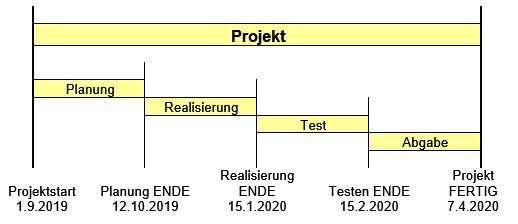
\includegraphics[height=6cm]{Images/Latex1.png}
	\end{figure}
	\label{Abbildung1}
	
	\section{Planung}
	\begin{figure}[ht]
		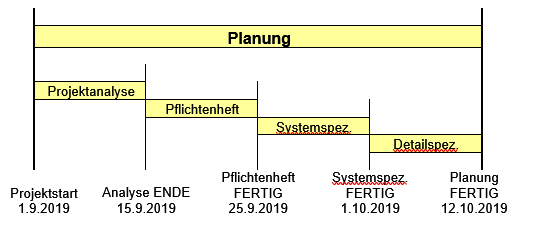
\includegraphics[height=6cm]{Images/Latex2.png}
	\end{figure}
	\label{Abbildung2}
	
	\section{Realisierung}
	$<$Termine für alle Phasen aus dem Gesamtprojektplan ...$>$

	\chapter{Umfeldanalyse}
	\section{$<$Was wird analysiert$>$}
	{$<$Beschreibung$>$}
	\subsection{Auswahlkriterien}
	\begin{itemize}
		\item $<$Kriterium 1$>$
		\item $<$Kriterium 2$>$
		\item Kosten
	\end{itemize}
	\subsection{$<$Alternative A $>$}
	\subsubsection{$<$Kriterium 1$>$}
	$<$Analyse Ergebnis$>$
	\subsubsection{$<$Kriterium 2$>$}
	$<$Analyse Ergebnis$>$
	\subsubsection{Kosten}
	$<$Analyse Ergebnis$>$
	\subsection{$<$Alternative B$>$}
		\subsubsection{$<$Kriterium 1$>$}
	$<$Analyse Ergebnis$>$
	\subsubsection{$<$Kriterium 2$>$}
	$<$Analyse Ergebnis$>$
	\subsubsection{Kosten}
	$<$Analyse Ergebnis$>$
	
	\subsection{Entscheidung}
	$<$Begründung$>$
	

	\chapter{Systemspezifikation}
	\section{Blockschaltbild}
	\begin{figure}[ht]
	{Images/1}
	\end{figure}
    \captionof{figure}{Blockschaltbild}
    \label{Abbildung}
	\section{Systemüberblick}
	\subsection{Funktionalität der Baugruppen}
	\subsubsection{Baugruppe I}
	$<$Beschreibung der Baugruppe I$>$
	\subsubsection{Baugruppe II}
	$<$Beschreibung der Baugruppe II$>$
	\section{Externe Schnittstellen}
	\subsection{$<$Schnittstelle A$>$}
	$<$Beschreibung der Schnittstelle A$>$
	\subsection{$<$Schnittstelle B$>$}
	$<$Beschreibung der Schnittstelle B$>$


	\chapter{Use Cases [OPTIONAL]}
	\section{Use Case $<$Name des Use Case$>$}
	Erklärung was der erste Anwendungsfall für eine Funktionalität bietet.
    \section{Use Case $<$Name des Use Case$>$}
    	Erklärung was der zweite Anwendungsfall für eine Funktionalität bietet.


	\chapter{Detailspezifikation [OPTIONAL]}
	\section{Detailspezifikation $<$Abc$>$}
    \subsection{$<$Detail 1$>$}
    $<$Beschreibung von Detail 1$>$\\
    \textcolor{red}{$<$UseCases ODER Struktogramme ODER Flussdiagramme ODER …$>$}
    \subsection{$<$Detail 2$>$}
   $<$Beschreibung von Detail 2$>$\\
   \textcolor{red}{$<$UseCases ODER Struktogramme ODER Flussdiagramme ODER …$>$}
    \section{Detailspezifikation $<$Xyz$>$}
    \subsection{$<$Detail 998$>$}
    $<$Beschreibung von Detail 998$>$\\
   \textcolor{red}{$<$UseCases ODER Struktogramme ODER Flussdiagramme ODER …$>$}
    \subsection{$<$Detail 999$>$}
    $<$Beschreibung von Detail 999$>$\\
   \textcolor{red}{$<$UseCases ODER Struktogramme ODER Flussdiagramme ODER …$>$}
    \section{Interne Schnittstellen}
    \subsection{$<$Schnittstelle S$>$}
    $<$Beschreibung der Schnittstelle S$>$
    \subsection{$<$Schnittstelle T$>$}
    $<$Beschreibung der Schnittstelle T$>$


\pagestyle{scrheadings}
\clearscrheadfoot

	\chapter{Benutzerhandbuch}
	\section{Benutzerhandbuch $<$Teil Abc$>$}
	\section{Benutzerhandbuch $<$Teil Abc$>$}


	\chapter{Testfallspezifikation}
	\section{Testgruppe $($Betriebsbereitschaft$)$}
	\subsection{Testfall $<$A$>$}
	\underline{\textbf{Randbedingung:}}
	\\
	\\
	$<$Randbedingungen$>$
	\\
	\\
	\underline{\textbf{Testablauf: }}
	\\
	\\
	$<$Eingabe(n) / Aktionen$>$
	\\
	\\
	\underline{\textbf{Erwartetes Ergebnis: }}
	\\
	\\
	$<$Welche Ausgabe / Aktion / Zustand soll erreicht werden$>$
	\subsection{Testfall $<$B$>$}
	\underline{\textbf{Randbedingung:}}
	\\
	\\
	$<$Randbedingungen$>$
	\\
	\\
	\underline{\textbf{Testablauf: }}
	\\
	\\
	$<$Eingabe(n) / Aktionen$>$
	\\
	\\
	\underline{\textbf{Erwartetes Ergebnis: }}
	\\
	\\
	$<$Welche Ausgabe / Aktion / Zustand soll erreicht werden$>$


\chapter{Begleitprotokoll}
In einem Begleitprotokoll sind der Arbeitsablauf $($zeitliche Auflistung, wann und wie lange an der abschließenden Arbeit gearbeitet wurde$)$ sowie die verwendeten Hilfsmittel und Hilfestellungen zu dokumentieren. Jedes Teammitglied ist verpflichtet, selbstständig sein eigenes Begleitprotokoll zu führen. Das Begleitprotokoll ist der schriftlichen Arbeit beizulegen $($§ 9 Abs. 2 Prüfungsordnung BMHS$)$.
\\
\noindent In der Rubrik Erstellung finden Sie eine Begleitprotokoll-Vorlage sowie Erläuterungen zum Begleitprotokoll. Sprechen Sie aber mit Ihrem Betreuer/Ihrer Betreuerin, ob Sie dieses Begleitprotokoll als Vorlage verwenden können.\\
\begin{large} Quelle:\url{http://www.diplomarbeiten-bbs.at/faq/faq-schuelerinnen}
\end{large}
\\
\noindent
Im Begleitprotokoll, das als Nachweis von Tätigkeiten, Meetings und Entscheidungen während der Diplomarbeit gilt, sind laufend Aufzeichnungen von den Schülerinnen bzw. von den Schülern zu führen. 
Dazu gibt es mehrere Möglichkeiten: 
\begin{itemize}
	\item das auf der DA-Webseite $($http://www.dipolmarbeiten-bbs.at$)$ vorgeschlagene Formular „Begleitprotokoll“ oder 
	\item die Projektmanagement Tools $($mit Taskverwaltung, Zeittracking und Meeting-Protokollen$)$ oder 
	\item die digitale Ablage in einem Dokumentenverwaltungssystem $($z. B. Dropbox usw.$)$ 
\end{itemize}
Die gewählte Form ist mit der Betreuerin bzw. dem Betreuer abzuklären und beinhalte folgende Aufzeichnungen: 
\begin{itemize}
	\item Dokumentation wichtiger Entscheidungen und Ereignisse, 
	\item Teambesprechungen deren Inhalte und Beschlüsse, 
	\item Besprechungen mit Betreuerinnen und Betreuern, 
	\item Dokumentation des individuellen Zeitaufwandes, 
	\item Kontakt zu Sponsoren, Investoren und Partnern. 	
\end{itemize}
Alle Inhalte müssen korrekt und vollständig dokumentiert sein. Auf Wunsch der Betreuerin bzw. des Betreuers sind die Aufzeichnungen jederzeit vorzulegen. 
Diese Aufzeichnungen dienen als: 
\begin{itemize}
	\item Nachweis von Tätigkeiten und Besprechungen, 
	\item Nachweis der Betreuungstätigkeit, 
	\item Überblick und Nachvollziehbarkeit von wichtigen Entscheidungen, 
	\item Nachvollziehbarkeit des Informationsflusses.
\end{itemize}
Quelle:	\url{http://www.diplomarbeiten-bbs.at/erstellung}\\
{\large{\textbf{Vorschlag $\rightarrow$}} Monatliche Zeit-Übersicht auf Basis der Wochenberichte
\section{Begleitprotokoll $<$Schüler 1$>$}
\begin{tabular}
{|c|l|r|}
\hline
{\textbf{Zeitraum}} &  Arbeiten / Tätigkeiten / Meetings / … & Stunden\\
\hline
2019/08 & & \\
\hline
2019/09 & & \\
\hline
2019/10 & & \\
\hline
2019/11 & & \\
\hline
2019/12 & & \\
\hline
2020/01 & & \\
\hline
2020/02 & & \\
\hline
2020/03 & & \\
\hline
2020/04 & & \\
\hline
\end{tabular}
\section{Begleitprotokoll $<$Schüler 2$>$}
\section{Begleitprotokoll $<$Schüler 3$>$}

%
	\chapter{Anhang}
	\section{Istbestand}
	\section{Angebote}
	\section{Lieferscheine}
	\section{Dimensionierung}
	\section{Messprotokolle}
	\section{Testprotokolle}
	\begin{tabular}
		{|R{4cm}|L{6cm}|R{2cm}|R{3cm}|}
		\hline
		Dokument: & \multicolumn{3}{l|}{{\huge\textbf{ Testprotokoll}}}\\
		\hline
		Projekt: & \multicolumn{3}{l|}{\huge\textbf {$<$DA-Name$>$}} \\
		\hline
		Version: & & Datum: & \\
		\hline
	\end{tabular}
    \\
    \noindent
    \begin{tabular}
    	{|R{4cm}L{4cm}R{3cm}R{4cm}R{2.7cm}|}
    	\hline
    	\multicolumn{4}{|l}{Gilt für:} &\\
    	\hline
    	Testfallbeschreibung: & \multicolumn{3}{|l}{\textbf{Diplomarbeit Kapitel 10} Testfallspezifikation} &\\
    	\hline
    	Test-Objekt: & \multicolumn{3}{|l}{\textbf{$<$DA-Name$>$ Prototyp}} &  \\
    	\hline
    \end{tabular}
    \\
    \noindent
    \begin{tabular}
    	{|R{4cm}|L{6cm}|L{5.4cm}|}
    	\hline
    	&  Name: &   Abteilung:\\
    	\hline
    	Test-Leiter: &  & Elektronik und Technische Informatik \\
    	\hline
    	Tester: & & Elektronik und Technische Informatik \\
        \hline
    \end{tabular}
    \\
    \noindent 
    \begin{tabular}
        {|C{1cm}C{1cm}|C{3cm}|C{4cm}|C{4.2cm}|}
        \hline
        \multicolumn{1}{|r}{Testfall} & & Datum / Zeit & Status & Bemerkungen \\
        & & & OK/not OK &   \\
        \hline	
        \multicolumn{1}{|l}{Testfall$<$A$>$} & & & OK & \\
        \hline	
        \multicolumn{1}{|l}{Testfall$<$B$>$} & & & OK & \\
        \hline        
    \end{tabular}   	


\appendix

%%================ Abkuerzungsverzeichnis ==============%%
%% start of file abkuerzungen.tex

% Abkuerzungsverzeichnis
\addchap{
	\iflanguage{english}{Acronyms}{Abkürzungsverzeichnis}}
\begin{acronym}[ACRONYM]
\acro{tikz}[TikZ]{\TikZ{} ist kein Zeichenprogramm}
\acro{spi}[SPI]{Serial Peripheral Interface}
\end{acronym}\newpage

%% end of file abkuerzungen.tex
%%======================================================%%


%%================ Abbildungsverzeichnis ===============%%
\setcounter{lofdepth}{2}
\dipalistoffigures
%%======================================================%%

%%================ Tabellenverzeichnis  ================%%
\setcounter{lotdepth}{2}
\dipalistoftables
%%======================================================%%

%%================ Literaturverzeichnis ================%%
\newpage
%% start of file literatur.tex

%% Literaturverzeichnis:
\begin{Literatur}
% The TeXbook by D. E. Knuth
\bibitem[1]{TeXbook}{\textbf{Donald~E.~Knuth:} \emph{The \TeX{}book}. 1986, {\scshape Addison--Wesley} Verlag,\\
ISBN-13: 978-0-201-13447-6} 
%
\end{Literatur}

%% end of file literatur.tex
 
	 
%%======================================================%%
\end{document}
